\definecolor{grey}{HTML}{CCA3A3}

\begin{figure}[H]
\center

\includegraphics[width=0.2\textwidth]{elasticsearch.png}
\label{fig:elasticsearchlogo.png}
\end{figure}
%\begin{wrapfigure}{r}{0.25\textwidth}
%\begin{center}
%
\includegraphics[width=0.25\textwidth]{elasticsearch.png}
%\end{center}
%\caption{A gull}
%\end{wrapfigure}
\section{Présentation de Elasticsearch}
Elasticsearch est moteur de recherche et d'analyse en temps réel. Il permet l'exploration
de données de façon très rapide par des recherches, que ce soit par des recherches
\gls{fulltext}, ou bien des recherches structurées.

Elasticsearch est depuis peu développé par la société \emph{Elastic}. C'était, à 
la base, un projet du développeur Shay Banon, qui souhaitait concevoir une API simplifié
pour la bibliothèque de moteur de recherche : Apache Lucene\fnu[Page du projet Lucene ]{https://lucenenet.apache.org/}.

Elasticsearch et la stack ELK est en passe de devenir un standard dans l'industrie.
En effet le logiciel à une utilisation assez versatile, de l'aide à la prise de 
décision en temps réelle à l'analyse de code source. Et à l'heure actuelle, la capacité 
à exploiter les masses de données et de méta données accumulées chaque jour devient 
un enjeu économique majeur (mais pas seulement \ldots). Enfin l'un des principaux 
atouts d'Elasticsearch réside dans son aptitude à pouvoir passer à l'échelle simplement.

\footnotesize{\emph{Attention, ce chapitre ne sera qu'une présentation très succinte des possibilités 
du logiciel Elasticsearch, tout détailler nécessiterait \emph{sans doutes} des milliers
de pages, le résumé officiel\footnote{Elasticsearch : The Definitive Guide, disponible 
chez Pearson et Github https://github.com/elastic/elasticsearch-definitive-guide}
en fait déjà \emph{plus de 950} \ldots}}

\section{Installation}
Avant même de regarder les différentes dépendances nécessaires à l'utilisation de
Elasticsearch il est recommandé de vérifier que l'on utilise bien la même version
que son compère Logstash (vérifier la compatibilité dans la documentation si les
versions de Logstash et Elasticsearch ont un numéro différent).

Son installation est sensiblement la même que son comparse logstash puisque ce logiciel 
nécessite également l'installation des dépendances \emph{jruby} et \emph{openjdk-7-jre}
à noter qu'il fonctionne également sur openjdk-8-jre.

Là aussi les paquets debian officiels n'existant pas on utilisera celui fourni par 
\href{https://download.elastic.co/elasticsearch/elasticsearch/elasticsearch-1.5.1.deb}{elastic.co}.
Et ici aussi le paquet est un peu approximatif puisqu'il faut rajouter certains 
chemin, et ajouter des droits.

\subsection{Configuration de base}


Acompleter et revoir
p24-26
 test


\section{Sense}
Sense est un module chrome développé par Boaz Leskes, il sert de front-end à ElasticSearch.
Le développement (public) de ce module est maintenant arrêté. Il fait parti de 
\emph{Marvel} le logiciel de monitoring et d'optimisation, vendu\footnote{voir bas 
de page : \url{https://www.elastic.co/products/marvel/signup.html}} 
par la société \emph{elastic}.


\subsection{Installation}
Installer ce logiciel est simple comme installer une extension Chrome\footnote{testé sur chromium}
tierce.
Tout d'abord : récupérer le module à l'adresse \url{https://github.com/bleskes/sense}
en utilisant par exemple : 
\begin{lstlisting}[style=code,label=lst:gitclonesense]
git clone https://github.com/bleskes/sense.git
\end{lstlisting}

Il suffit ensuite de l'activer dans chromium :\\ 
chrome://extension => Developer mode => Load unpacked extension.

\begin{figure}[H]
\center
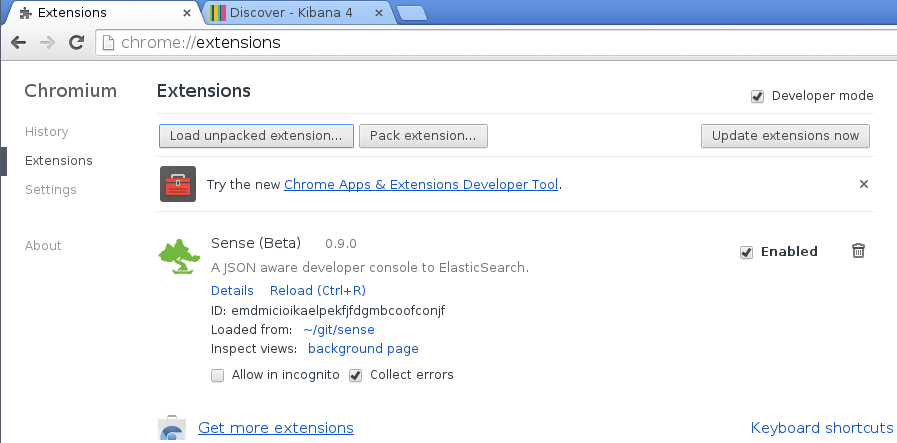
\includegraphics[width=12cm]{senseinstall.png}
\label{fig:senseinstall}
\caption{Plugin Sense installé dans chromium}
\end{figure}

Et voilà ! \footnotesize{(avec un accent anglais)}

\subsection{Utilisation de Sense}
L'utilisation de Sense est assez simple via son interface :

\begin{figure}[H]
\center
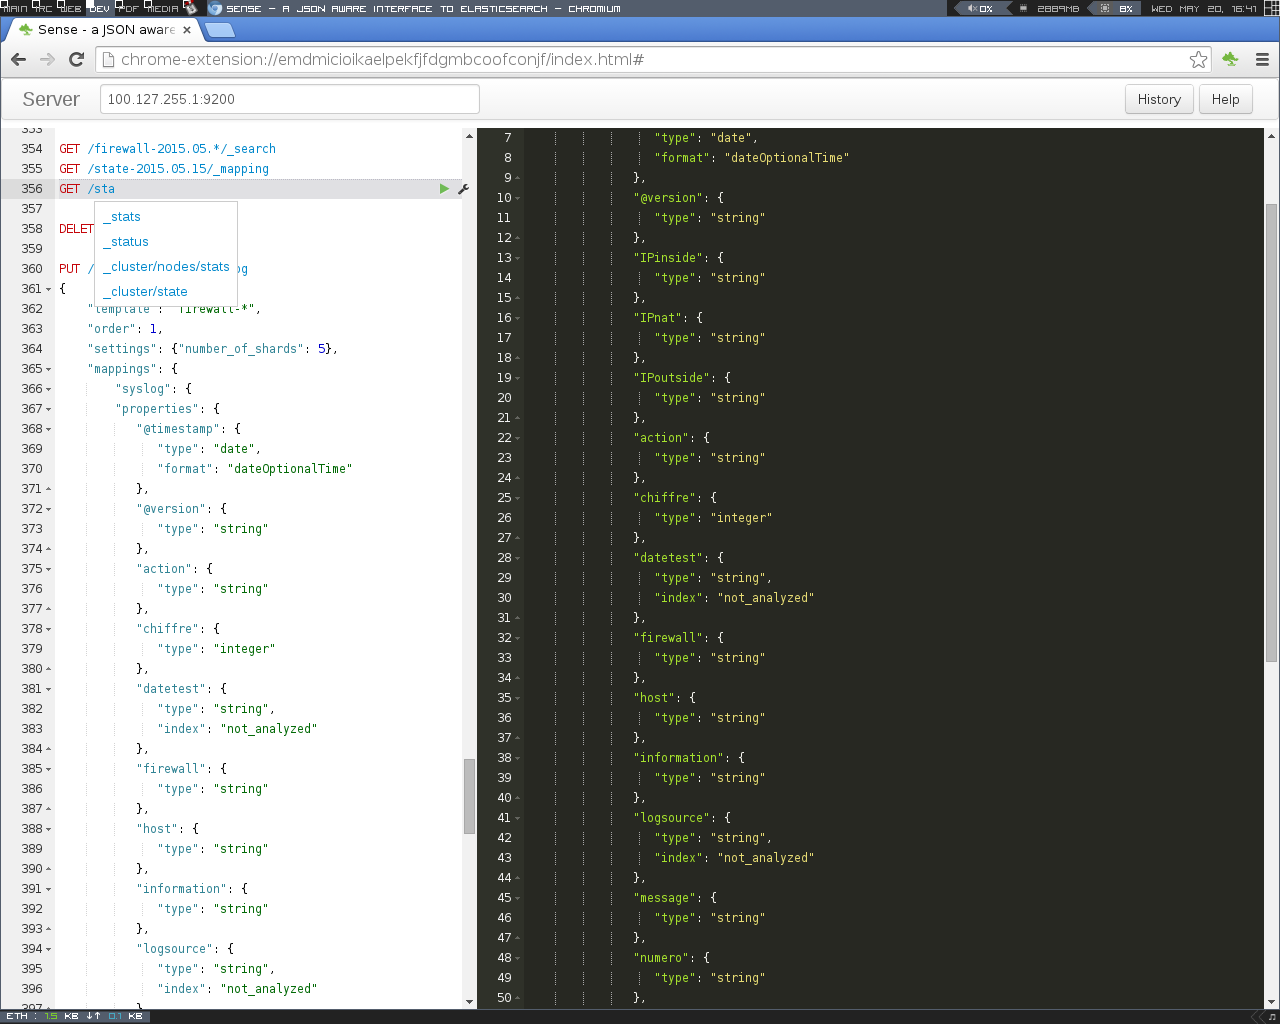
\includegraphics[width=15cm]{sensegui.png}
\label{fig:sensegui.png}
\caption{Vue générale de Sense}
\end{figure}

La difficulté se situe évidemment plutôt du coté de l'appréhension, la configuration
et l'optimisation de Elasticsearch.

Nous allons avec l'image ci-dessous \ref{fig:sensegui2.png} brièvement expliquer le fonctionnement de Sense
\begin{figure}[H]
\center
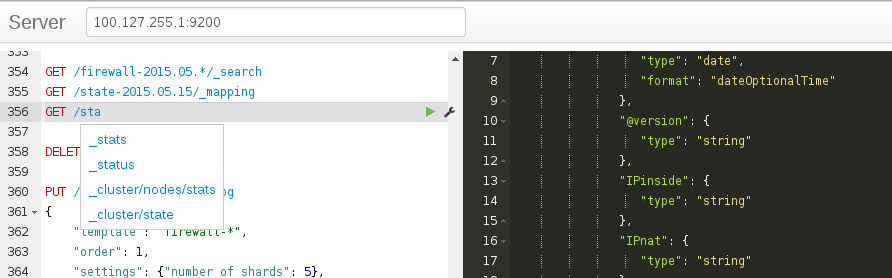
\includegraphics[width=15cm]{sensegui2.png}
\label{fig:sensegui2.png}
\caption{Zoom sur les fonctionnalités de Sense}
\end{figure}
Le formulaire \textbf{Server} situé en haut correspond à l'adresse et au port d'écoute 
de l'instance Elasticsearch sur laquelle on souhaite travailler.

Le panneau de gauche correspond au \textbf{panneau de requête}. On utilise l'api REST d'elasticsearch
pour envoyer des requêtes (recherches, modification etc, point sur l'API prévu 
ultérieurement). Il est à noté que le panneau de gauche est doté d'une autocomplétion
pour les fonctions et configurations standards dans elasticsearch.

Le panneau de droite est le \textbf{panneau de réponse} aux requêtes. Les informations
nous parviennent en JSON.

\section{La théorie}

\subsection{Approximation et comparaison avec le modèle relationnel}
La comparaison entre Elasticsearch et une base de données n'est pas forcement heureuse,
c'est un moteur de recherche (d'indexation). Il utilise donc la notion d'index   
qu'on peut cependant assez facilement comparer au modèle relationnel.

Elasticsearch s'organise autour d'index que l'on peut comparer aux bases (de données)
dans le modèle relationnel, un index peut utiliser plusieurs types (dans notre projet
nous aurions pu différencier les logs firewall des logs \textit{states} en utilisant 
les types), les types s'apparentent aux tables dans le modèle relationnel. 
Chaque enregistrement d'Elasticsearch est effectué sous forme document. Les documents
(qui ont un type, éventuellement type par défaut), un document peut être comparé 
à une ligne, ou un enregistrement. Ces lignes sont constitués de colonnes, appellées
champs (ou fields) dans Elasticsearch.


{\Huge NEED image}

\section{L'infrastructure}

\subsection{Le tunning}
Voici quelques conseilles qui sont applicables pratiquement dans toutes les situations
pour une utilisation optimale de Elasticsearch.

\subsubsection{Ne pas utiliser la swap}
Il est très fréquent (et souvent nécessaire) de formater une partition de swap pour
que le système puisse optimiser son fonctionnement. C'est très pratique pour ne pas
saturer la mémoire RAM de nos machines de bureau, notamment quand on voit la consommation
pantagruélique de certains navigateurs internet récents. Les fichiers qui ne sont 
susceptible de ne pas être utilisé avant un long moment sont parfois stocké sur le
disque dur afin de libérer de l'espace pour d'autres applications, la swap est
également utilisé lorsque l'on met un ordinateur en veille \ldots

La situation n'est pas la même sur un serveur. Ici nous sommes relativement maitre
de notre environnement, et de plus nous voulons que le service Elasticsearch soit 
le plus véloce possible, pour se faire il faut au contraire l'empêcher au maximum 
d'utiliser la partition de swap (forcément plus lente).

Il existe plusieurs façon de faire (y compris ne pas utiliser de partition de swap)
celle que j'ai choisie d'utiliser est de modifier la variable \ipath{vm.swapiness}
dans le fichier \ipath{/etc/sysctl.conf}. La swapiness représente le pourcentage
de mémoire RAM restant à partir duquel on commence à envoyer de informations en
swap.

\begin{lstlisting}[style=code,label={lst:configswapiness},caption={Configuration swapiness}]
vm.swapiness = 2
swapoff -a
swapon -a
\end{lstlisting}
Il existe deux méthodes pour que le changement de swapiness soit pris en compte :
redémarrer la machine ou bien désactiver puis réactiver la swap, via les commandes
swapon, swapoff. Utiliser la commande swapoff est également une mesure radicale à 
notre problème.

\subsubsection{Utiliser une quantité de RAM raisonné}
Elasticsearch est limité par Java. Avant de parler de ces limites, il faut rappeler 
que Elasticsearch est un front-end à Apache Lucene. Lucene est conçu pour tirer 
parti très efficacement du cache des système de fichiers (probablement ext4 si 
vous utilisez Debian), qui sont en définitif, gérer par le 
noyau\footnote{https://www.elastic.co/guide/en/elasticsearch/guide/current/\_limiting\_memory\_usage.html}.
Il est conseillé par la documentation de donner au maximum 50\% de la mémoire RAM
disponible à Elasticsearch, le reste étant dévouer à lucène et au bon fonctionnement
du système.
Dans notre installation dont nous parlerons plus en détail ultérieurement, nous 
avons choisi de nous réserver une bonne marge de manœuvre puisqu'un redis et un Logstash
minimalistes tournent en sus sur la machine hébergeant Elasticsearch.

Cependant cette valeur de 50\% n'a de sens que si Elasticsearch consomme moins de 
32Go de RAM, en effet, en allouer plus devient contreproductif puisque jusqu'à 32Go
la machine virtuelle Java (JVM) \textit{compresse} les adresses des pointeurs, 
(tant qu'on reste sous la limite des 32Go de RAM on peut continuer à utiliser les 
adresses mémoires sur 4 octets), après, la consommation de mémoire explose et le
\textit{garbage collector} devient bien moins efficace.

Pour les machines possédant une énorme quantité de mémoire RAM (128Go à 1To)
il conseiller pour optimiser le fonctionnement de la machine de faire tourner plusieurs
noeuds d'Elasticsearch dessus (attention aux entrées sortie et à l'utilisation processeur
cependant.

\section{Les API Elasticsearch}
Elasticsearch est énorme, mais être assez facilement utilisable par le 
plus grand nombre, des \gls{API} \emph{optimisées} pour chaque tâches ont été conçues.

\subsection{API REST}
Cette API sert à la communication avec Elastisearch, comme toutes les API REST elle
utilise les méthodes HTTP, ici : GET, POST, PUT et DELETE et s'appuie ensuite sur l'architecture d'Elasticsearch.

\textbf{{\color{grey}http://host:port}/[{\color{red}index}]/[{\color{cyan}type}]/[{\color{yellow}\_action/id}]}\\[5mm]
Imaginons que dans un projet fictif, nous souhaitions référencer des tweets.
On pourrait procéder comme suit pour ajouter le premier.

\textbf{PUT  {\color{grey} http://100.127.255.1:9200}/{\color{red}twitter}/{\color{cyan}tweet}/{\color{yellow}1}}

\begin{lstlisting}[style=code,label={lst:RESTexemple1curl},caption={Avec curl}]
curl -XPUT http://100.127.255.1:9200/twitter/tweet/1
\end{lstlisting}
Voici le résultat en utilisant curl, directement en ligne de commande, par 
navigateur, \ldots

\begin{lstlisting}[style=code,label={lst:RESTexemple1sense},caption={Avec Sense}]
PUT /twitter/tweet/1
\end{lstlisting}

Voici la syntaxe que nous obtiendrions en utilisant Sense, puisque notre serveur 
et notre port sont déjà renseignés, la syntaxe est bien plus courte.

La directive PUT est utilisé pour renseigner de nouvelles informations dans Elasticsearch.


Dans notre projet d'analyse de logs, il est fréquent que nous dussions supprimer 
des index, notamment dans le cas du paramétrage des \emph{mappings}, mais également
pour soulager notre infrastructure du poids des logs de firewall (~20-30Go/jours).\\

\textbf{DELETE  {\color{grey} http://100.127.255.1:9200}/{\color{red}twitter}/}\\

Si nous avions un index twitter journalier il serait possible d'utiliser une commande
très similaire pour supprimer tous les indexs d'un seul coup :\\

\textbf{DELETE  {\color{grey} http://100.127.255.1:9200}/{\color{red}twitter*}}\\

La directive DELETE est utilisé pour supprimer des informations d'Elasticsearch.\\


Enfin la directive GET qui sert à récupérer des information, à tout niveaux, index,
type, mapping, type par défaut \ldots, en revanche il faut avoir un identifiant exact,
ce n'est pas un outils de recherche (abordé dans la section suivante).\\[5mm]
\textbf{GET  {\color{grey} http://100.127.255.1:9200}/{\color{red}twitter}/{\color{cyan}tweet}/{\color{yellow}1}}\\

Les information récupérées le sont en JSON.

\subsection{QueryDSL}
DSL pour Domain Specific Language, parce que Elasticsearch est avant tout un moteur 
de recherche, il dispose de puissantes fonctionnalités de recherche. Il dispose donc
de son propre langage d'interrogation le QueryDSL. C'est loin d'être un cas unique,
par exemple Puppet dispose également de son propre langage de configuration.

Il existe une QueryDSL restreint et un QueryDSL étendu.
%\subsubsection{}



\section{Le mapping}
